\section{Reprodução}
\label{sec:reproducao}

\subsection{Artefatos e ambiente}
O pacote de artefatos (selos \emph{Available} e \emph{Evaluated -- Functional}) contém os 30 modelos \uvl{}, as 150 respostas da API do Codex, os textos e embeddings enviados à Cohere e um notebook do Google Colab. Como o Codex foi desativado, a reprodução usa as respostas guardadas.

\paragraph{Problemas encontrados no ambiente.} O notebook não executa como publicado: \todo{revisar}
\begin{itemize}
  \item a versão atual do \flamapy{} (2.x) não lê 26 dos 30 modelos originais; foi necessário fixar as versões de 2023 (\texttt{flamapy~1.1.3}, \texttt{flamapy-fm~1.1.3}, \texttt{flamapy-sat~1.1.7}, \texttt{flamapy-bdd~1.0.1}), esta última com metadados inválidos no PyPI;
  \item a operação de \emph{false-optional features} mudou de assinatura entre versões do \texttt{flamapy-sat};
  \item a célula de inferência contém erro de sintaxe e usa a API da OpenAI anterior à versão 1.0;
  \item variáveis indefinidas (\texttt{DIRECTORY\_UVL}) e importações ausentes (\texttt{cohere}, \texttt{time}, \texttt{random}) nos experimentos 2 e 3;
  \item o prompt enviado ao Codex era a representação textual de uma lista Python (\texttt{str(list)}), não o texto do modelo.
\end{itemize}
O ambiente corrigido (Python 3.12) e um notebook atualizado estão no repositório do grupo.

\subsection{Resultados da reprodução}
\Cref{tab:reproducao} compara os números do artigo com os obtidos.

\begin{table}[t]
  \caption{Artigo original versus reprodução (dados publicados).}
  \label{tab:reproducao}
  \small
  \begin{tabular}{lrr}
    \toprule
    Medida & Artigo & Reprodução \\
    \midrule
    Variantes sintaticamente válidas & 136/150 & 136/150 (90,7\%) \\
    Respostas do Codex vazias & --- & 38/150 \\
    Similaridade mediana (orig.\ vs.\ variante) & 0,5--0,8\textsuperscript{*} & 0,943 \\
    Variantes com similaridade em [0,5; 0,8] & ``maioria'' & 27/150 \\
    Variantes com similaridade = 1,0 & --- & 29/150 \\
    Variantes com similaridade $<$ 0,5 & --- & 0/150 \\
    \bottomrule
  \end{tabular}\\[2pt]
  \footnotesize\textsuperscript{*}faixa relatada para ``a maioria'' das variantes.
\end{table}

As 14 variantes inválidas concentram-se em poucos modelos: todas as 5 de \texttt{aircraft\_fm} e de \texttt{REAL-FM-2}, 2 de \texttt{REAL-FM-12}, 1 de \texttt{REAL-FM-17} e 1 de \texttt{REAL-FM-6}. \todo{classificar os erros (tabulação vs.\ relação sem tipo) e comparar com o artigo.}

\begin{figure*}[t]
  \centering
  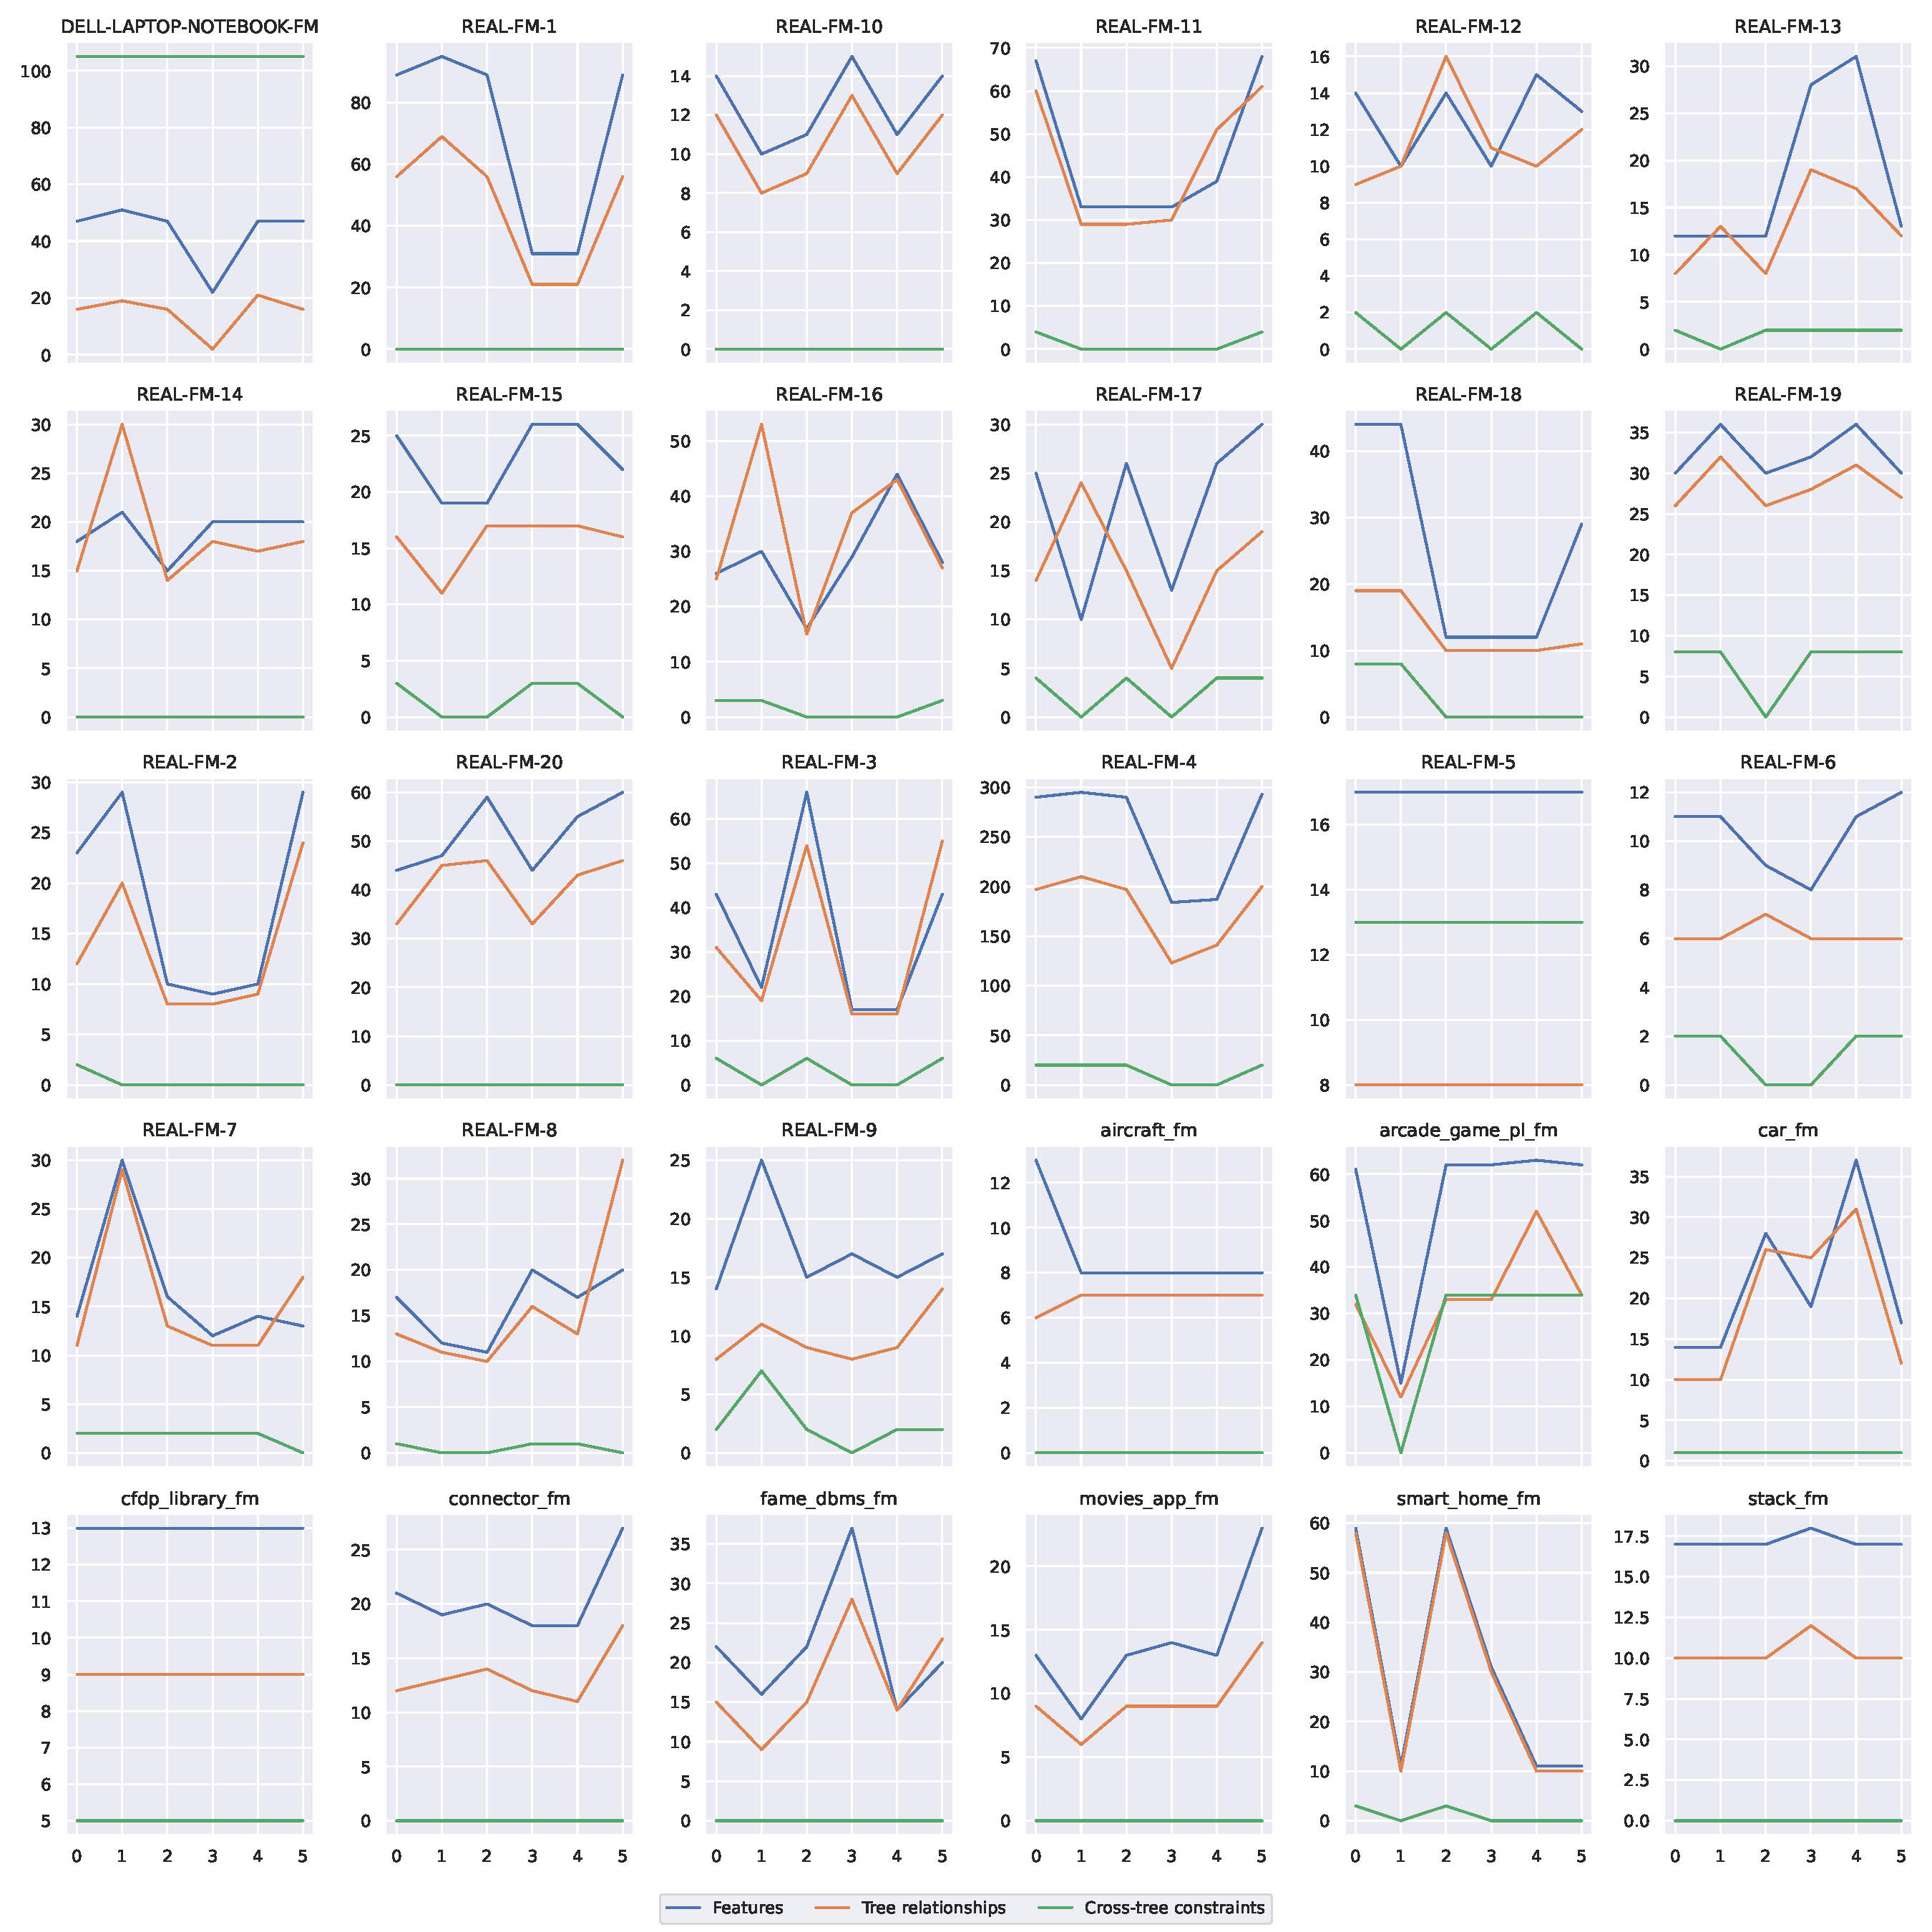
\includegraphics[width=.8\textwidth]{semantics_structure.pdf}
  \caption{Reprodução do experimento 2: features, cross-tree constraints e relações por iteração (0 = original).}
  \label{fig:estrutura}
\end{figure*}

\paragraph{Discrepância na similaridade de domínio.} \todo{discutir: a métrica premia cópias (resposta vazia $\Rightarrow$ 1,0) e penaliza variantes que perdem features; motiva o funil da replicação.}
